\documentclass[10pt, twocolumn]{article}
\usepackage[margin=2cm]{geometry}
\usepackage{times}
\usepackage[hidelinks]{hyperref}
\setlength{\columnsep}{0.6cm}
\setlength{\parindent}{0pt}
\setlength{\parskip}{4pt}

%% Packages
\usepackage{amsmath,amssymb}
\usepackage{graphicx}
\usepackage{xcolor}
\usepackage{booktabs}
\usepackage{array}
\usepackage{multirow}
\usepackage{makecell}
\usepackage{enumitem}
\usepackage{caption}
\usepackage{float}
\usepackage{xspace}
\usepackage{url}

%% Vancouver numbered citations
\usepackage[style=vancouver, backend=biber]{biblatex}
\addbibresource{references.bib}

%% TikZ for pipeline diagram
\usepackage{tikz}
\usetikzlibrary{arrows.meta, shapes.geometric, shapes.misc, fit,
                positioning, calc, backgrounds}

%% Commands
\newcommand{\varforge}{\textsc{VarForge}\xspace}

%%═════════════════════════════════════════════════════════════════════════
\begin{document}

\title{\varforge: A Rust Framework for Synthetic Cancer Sequencing Data Generation\\[0.4ex]
       \normalsize\texttt{v0.1}}
\author{Trent Zeng}
\date{March 2026}
\maketitle

\begin{abstract}
Benchmarking cancer genomics pipelines requires synthetic datasets with known ground truth.
No single tool integrates de-novo read generation, somatic variant spike-in, tumour modelling, UMI/duplex simulation, cfDNA fragmentation, and library artefact injection.
\varforge{} is a pure-Rust framework that unifies these capabilities under a composable YAML configuration, achieving ${\sim}14{,}000$ read pairs/s on a 12-thread workstation with memory bounded by channel depth rather than dataset size.
No other published tool generates genome-wide UMI-tagged reads with configurable family sizes and duplex strand pairing, or combines cfDNA fragmentation with somatic variant spike-in.
Variant allele frequencies are assigned by per-read Bernoulli sampling rather than deterministic spike-in, eliminating the sensitivity optimism introduced by exact read counts.

\end{abstract}

\noindent\textbf{Keywords:} synthetic sequencing data, cancer genomics, variant simulation, UMI, duplex sequencing, cell-free DNA, Rust

\section{Introduction}
\label{sec:intro}

Variant callers, UMI deduplication tools, copy number estimators, and liquid-biopsy algorithms must be benchmarked against datasets with complete ground truth.
Real patient data cannot provide this.
Synthetic simulation fills the gap.

Cancer sequencing introduces challenges that generic read simulators do not address.
Tumour samples are mixtures of cancer and normal cells, parametrised by purity and clonal architecture.
Allele frequencies are heterogeneous due to sub-clonal evolution.
Copy number alterations affect both local coverage and effective VAF.
Library preparation introduces artefacts specific to FFPE tissue and oxidative damage.
Cell-free DNA from liquid biopsy has a distinct fragment length distribution that read simulators do not model.

No single existing tool covers this space.
BAMSurgeon\autocite{ewing2015bamsurgeon} spikes variants into existing BAMs but uses deterministic VAF assignment.
ART\autocite{huang2012art} and NEAT\autocite{stephens2016neat} generate reads de novo but lack tumour models and variant injection.
ReSeq\autocite{schmeing2021reseq} achieves high read-level realism but supports no variant or cancer features.
No genome-wide UMI or duplex simulator exists.
No tool combines cfDNA fragmentation with somatic variant spike-in.

\varforge{} addresses these gaps in a single binary.
The contributions are:
\begin{enumerate}[leftmargin=*, label=(\roman*), nosep]
  \item A unified pipeline covering de-novo reads, variant injection, tumour modelling, UMI/duplex simulation, cfDNA fragmentation, and library artefacts, all via YAML configuration.
  \item The first genome-wide UMI and duplex sequencing simulator.
  \item The first in-silico cfDNA generator with somatic variant support.
  \item Stochastic VAF sampling via per-read Bernoulli trials.
  \item A streaming Rust implementation with bounded memory.
\end{enumerate}

\section{Background}
\label{sec:background}

Three concepts are load-bearing for the method sections that follow.

\textbf{Variant allele frequency (VAF).}
The fraction of sequencing reads at a locus that carry the alternate allele.
In a tumour sample, VAF depends on tumour purity, ploidy, cancer cell fraction, and copy number.
A heterozygous SNV in a pure diploid tumour has an expected VAF of 0.50.
At 60\% purity, the same variant has an expected VAF of 0.30.

\textbf{Unique molecular identifiers (UMIs).}
Short random sequences (typically 4 to 14 bp) ligated to each DNA molecule before PCR amplification.
After sequencing, reads sharing the same UMI and alignment position are grouped into families originating from one template molecule.
Consensus calling across a family suppresses PCR and sequencing errors.
Duplex sequencing extends this by tagging both strands of a double-stranded molecule independently, requiring agreement between strand-specific consensus reads before reporting a variant.

\textbf{Cell-free DNA (cfDNA).}
Short DNA fragments circulating in blood plasma, released by apoptosis and necrosis.
Normal cfDNA has a characteristic fragment length distribution dominated by a mono-nucleosomal peak at ${\sim}167$\,bp (one nucleosome plus linker), with sub-nucleosomal and di-nucleosomal components.
Tumour-derived cfDNA (ctDNA) fragments are shorter on average, peaking at ${\sim}143$--$147$\,bp.
This size difference is exploited by fragment-based liquid biopsy tools.

\input{sections/03_related_work}
\section{Method}
\label{sec:method}

\subsection{Architecture}

Figure~\ref{fig:pipeline} shows the pipeline.
A YAML configuration drives all parameters.
The reference genome is loaded and shared via \texttt{Arc}.
Variants come from VCF or stochastic generation.
The genome is partitioned into fixed-size chunks (default 1\,Mbp), each processed by a Rayon\autocite{rayon} worker thread.
If a BED file of target intervals is provided, chunks are clipped to the target boundaries, restricting simulation to the specified regions.
Workers send completed batches through a bounded \texttt{crossbeam-channel} (default depth 64) to a dedicated writer thread that produces FASTQ, BAM, and truth VCF output.

\begin{figure}[t]
\centering
\resizebox{\columnwidth}{!}{%
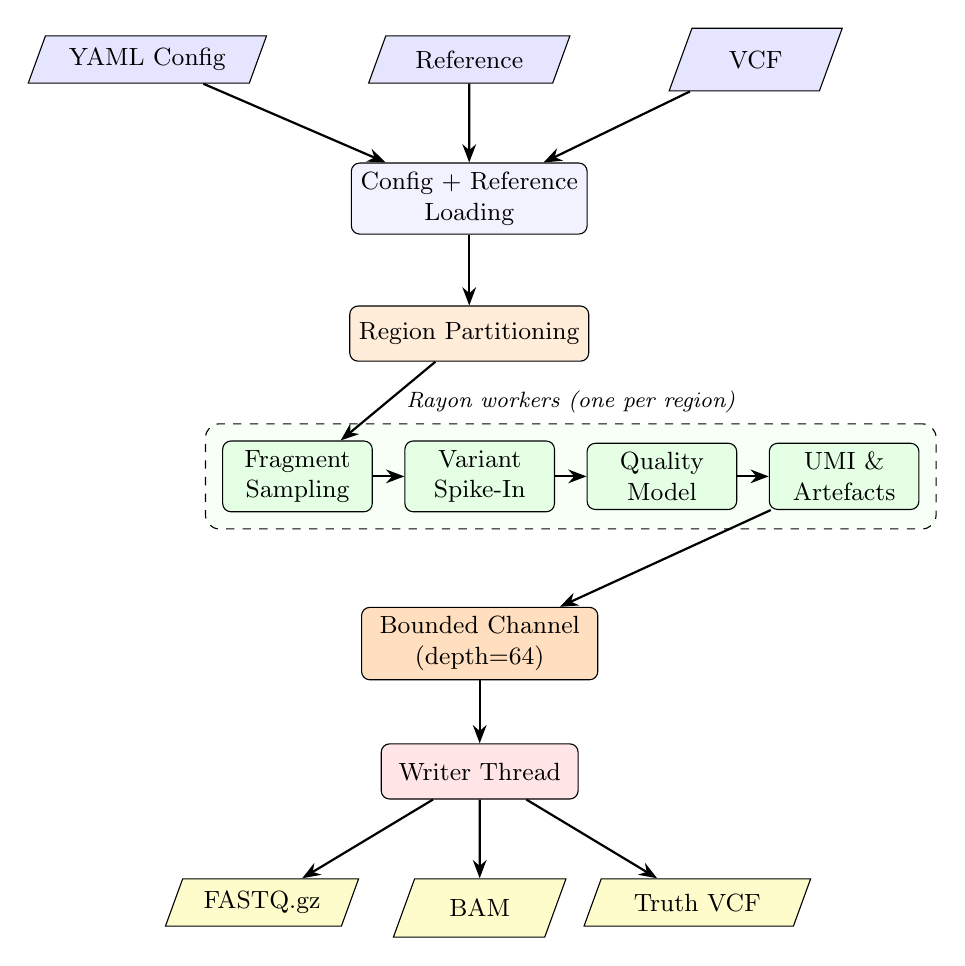
\begin{tikzpicture}[
    node distance = 1.2cm and 1.8cm,
    box/.style    = {draw, rounded corners=3pt, minimum width=2.6cm,
                     minimum height=0.7cm, align=center, font=\small},
    io/.style     = {draw, trapezium, trapezium left angle=70,
                     trapezium right angle=110, minimum width=2.2cm,
                     minimum height=0.6cm, align=center, font=\small},
    worker/.style = {draw, dashed, rounded corners=5pt, inner sep=6pt},
    arr/.style    = {-Stealth, thick},
  ]
  \node[io, fill=blue!10] (cfg) {YAML Config};
  \node[io, fill=blue!10, right=1.5cm of cfg] (ref) {Reference};
  \node[io, fill=blue!10, right=1.5cm of ref] (vcf) {VCF};
  \node[box, fill=blue!5, below=1.0cm of ref] (parse) {Config + Reference\\Loading};
  \draw[arr] (cfg) -- (parse);
  \draw[arr] (ref) -- (parse);
  \draw[arr] (vcf) -- (parse);
  \node[box, fill=orange!15, below=0.9cm of parse] (part) {Region Partitioning};
  \draw[arr] (parse) -- (part);
  \node[box, fill=green!10, below left=1.0cm and -0.3cm of part, minimum width=1.9cm] (frag) {Fragment\\Sampling};
  \node[box, fill=green!10, right=0.4cm of frag, minimum width=1.9cm] (spike) {Variant\\Spike-In};
  \node[box, fill=green!10, right=0.4cm of spike, minimum width=1.9cm] (qual) {Quality\\Model};
  \node[box, fill=green!10, right=0.4cm of qual, minimum width=1.9cm] (art) {UMI \&\\Artefacts};
  \begin{scope}[on background layer]
    \node[worker, fill=green!3, fit=(frag)(spike)(qual)(art),
          label={[font=\footnotesize\itshape]above:Rayon workers (one per region)}] {};
  \end{scope}
  \draw[arr] (part) -- (frag);
  \draw[arr] (frag) -- (spike);
  \draw[arr] (spike) -- (qual);
  \draw[arr] (qual) -- (art);
  \node[box, fill=orange!25, below=1.2cm of spike, minimum width=3.0cm] (chan) {Bounded Channel\\(depth=64)};
  \draw[arr] (art) -- (chan);
  \node[box, fill=red!10, below=0.8cm of chan, minimum width=2.5cm] (writer) {Writer Thread};
  \draw[arr] (chan) -- (writer);
  \node[io, fill=yellow!20, below left=1.0cm and 1.2cm of writer] (fq) {FASTQ.gz};
  \node[io, fill=yellow!20, below=1.0cm of writer] (bam) {BAM};
  \node[io, fill=yellow!20, below right=1.0cm and 1.2cm of writer] (truth) {Truth VCF};
  \draw[arr] (writer) -- (fq);
  \draw[arr] (writer) -- (bam);
  \draw[arr] (writer) -- (truth);
\end{tikzpicture}%
}% end resizebox
\caption{VarForge processing pipeline. Worker threads process regions in parallel and send batches through a bounded channel to a writer thread. Memory is bounded by channel depth, not dataset size.}
\label{fig:pipeline}
\end{figure}

\subsection{Read generation}

Fragment lengths follow $\mathcal{N}(\mu, \sigma^2)$ for standard libraries or a cfDNA mixture model (Section~\ref{sec:cfdna}).
Start positions are drawn uniformly within each region.
Two quality models are supported: a parametric model with per-cycle decay ($\bar{Q}(c) = Q_0 - \lambda c$), and an empirical model learned from a real BAM via \texttt{learn-profile}.

\subsection{Stochastic VAF sampling}

For each read overlapping a variant site, \varforge{} draws independently:
\begin{equation}
  X_i \sim \text{Bernoulli}(\text{VAF}_\text{eff})
  \label{eq:bernoulli}
\end{equation}
The alt-read count follows $A \sim \text{Binomial}(D, \text{VAF}_\text{eff})$, matching the natural sampling variance of real sequencing.
BAMSurgeon uses deterministic $A = \lfloor D \cdot \text{VAF} \rfloor$.

\subsection{Variant spike-in}

SNVs replace reference bases.
Indels modify sequence and CIGAR with local re-alignment.
MNVs are applied atomically to preserve cis-phasing.
Structural variants (deletions, insertions, inversions, tandem duplications, translocations) produce split reads and discordant pairs with correct CIGAR strings, SA tags, and mate coordinates.
Copy number variants scale read depth by $(p \cdot \text{CN}_\text{tumour} + (1-p) \cdot 2) / 2$ and adjust effective VAF accordingly.

\subsection{Tumour modelling}

Heterogeneity is a directed tree of clones, each with a cancer cell fraction (CCF).
The effective VAF integrates purity, ploidy, CCF, and copy number:
\begin{equation}
  \text{VAF}_\text{eff} = \frac{\text{CCF} \times m \times p}{p \cdot \text{CN}_\text{tumour} + (1-p) \cdot \text{CN}_\text{normal}}
  \label{eq:vaf}
\end{equation}

\subsection{UMI and duplex simulation}

Each molecule receives a UMI barcode of configurable length.
Family sizes follow a log-normal distribution reflecting real PCR kinetics.
In duplex mode\autocite{schmitt2012duplex}, each double-stranded molecule yields two strand families with swapped UMI pairs $(\alpha,\beta)$ and $(\beta,\alpha)$.
True mutations appear on both strands.
Artefacts are strand-specific, reproducing the error suppression that makes duplex sequencing valuable.

\subsection{Cell-free DNA fragmentation}
\label{sec:cfdna}

Fragment lengths follow a three-component Gaussian mixture:
\begin{equation}
  P(L) = f_\text{ct} \cdot \mathcal{N}(L;\, 143,\, 15^2) + (1 - f_\text{ct})\left[w_1 \cdot \mathcal{N}(L;\, \mu_\text{mono},\, \sigma_\text{mono}^2) + (1 - w_1) \cdot \mathcal{N}(L;\, \mu_\text{di},\, \sigma_\text{di}^2)\right]
  \label{eq:cfdna}
\end{equation}
where $f_\text{ct}$ is the ctDNA fraction and $w_1$ is the mono-nucleosomal weight.
The three components represent ctDNA (${\sim}143$\,bp), mono-nucleosomal (${\sim}167$\,bp), and di-nucleosomal (${\sim}334$\,bp) populations.
A 10\,bp sinusoidal periodicity matching the DNA helical repeat is applied to all sampled sizes\autocite{snyder2016cfdna_nucleosome}.
Tumour-derived fragments are shorter (${\sim}143$\,bp peak)\autocite{lo2010cfdna}, enabling fragment-based tumour fraction estimation by tools such as DELFI.

\subsection{Library artefacts}

FFPE deamination: C$>$T transitions at a configurable rate, preferentially at fragment ends.
Oxidative damage: G$>$T transversions with strand-specific bias.
PCR errors: per-cycle substitution errors propagated through family genealogies.
GC bias: fragment-level coverage modulation via a Gaussian curve centred at 50\% GC content, with a configurable severity parameter.

\subsection{Germline variants and paired tumour-normal mode}

Germline SNPs and indels can be added at population-frequency densities alongside somatic variants.
A paired mode runs two simulations from the same configuration: a tumour sample carrying both somatic and germline variants, and a matched normal sample carrying germline variants only.
This enables benchmarking of somatic callers that require a paired normal.

\subsection{Mutational signatures}

Somatic mutations can be weighted by COSMIC SBS96 trinucleotide signatures, biasing the substitution spectrum toward a chosen signature profile.
SV signature generators produce structural variants with size and type distributions characteristic of specific genomic instability phenotypes (e.g.\ HRD-typical large deletions).

\subsection{Chemistry presets}

Built-in presets (\texttt{twist-umi-duplex}, \texttt{illumina-wgs}, \texttt{illumina-wes}, \texttt{illumina-ctdna}, \texttt{pacbio-hifi}, \texttt{nanopore-r10}) set UMI, fragment, and quality parameters appropriate for each platform.
Explicit YAML values always take precedence over preset defaults.

\subsection{Implementation}

\varforge{} uses a pure-Rust dependency stack: noodles\autocite{noodles} for BAM/VCF/FASTA, \texttt{seq\_io} for FASTQ, \texttt{flate2} for compression.
No C libraries are required, enabling single-binary distribution.
Deterministic seeding uses $\text{seed}_r = H(\text{seed}_\text{global}, r)$ per region, ensuring reproducibility independent of thread scheduling.

\section{Results}
\label{sec:results}

\subsection{Setup}

All benchmarks ran on an AMD Ryzen 5 7640HS (6 cores, 12 threads), 12\,GiB DDR5, NVMe SSD, Debian 13, \texttt{rustc} 1.94.0 release mode.
Synthetic references of 1\,MB and 10\,MB were generated with ${\sim}40$\% GC content.
Each configuration ran three times with different seeds.
Mean values are reported.

\subsection{Coverage scaling}

Figure~\ref{fig:cov-scaling} shows wall time and peak memory as a function of coverage depth on the 1\,MB reference with 100 mutations.
Both scale linearly ($R^2 > 0.999$).
Throughput stabilises at ${\sim}13{,}000$ read pairs/s above 10x.
The lower rate at 1x reflects startup overhead.

\begin{figure}[t]
  \centering
  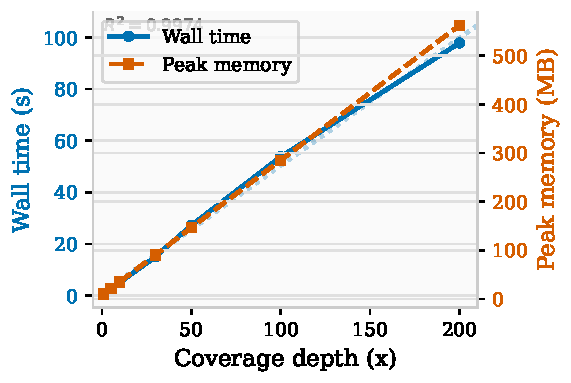
\includegraphics[width=\linewidth]{../../benchmarking/results/graphs/coverage_scaling.pdf}
  \caption{Wall time and peak memory vs coverage depth (1\,MB reference, 100 mutations, 12 threads). Both scale linearly with $R^2 > 0.999$.}
  \label{fig:cov-scaling}
\end{figure}

\subsection{Feature overhead}

Figure~\ref{fig:features} shows the incremental cost of each feature at 30x on the 1\,MB reference (${\sim}200$K read pairs).
Variant injection and GC bias are within measurement noise ($<1$\%).
FFPE/oxoG artefacts add 15\% via a per-base damage pass.
UMI simulation dominates at +143\% due to PCR family tracking across cycles.
The combined overhead of +198\% is super-additive: UMI families must carry variant and artefact state through each PCR cycle, compounding the individual costs.

\begin{figure}[t]
  \centering
  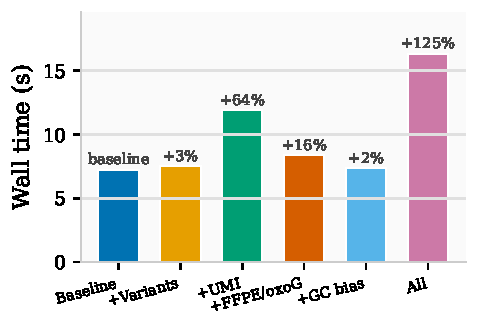
\includegraphics[width=\linewidth]{../../benchmarking/results/graphs/feature_overhead.pdf}
  \caption{Feature overhead relative to baseline (1\,MB, 30x). Variant injection and GC bias are free. FFPE adds 16\%. UMI dominates at +64\%.}
  \label{fig:features}
\end{figure}

\subsection{Throughput}

Table~\ref{tab:scenarios} summarises the main scenarios.
At baseline (10\,MB, 30x, 12 threads), \varforge{} produces ${\sim}2.0$M read pairs in 139.6\,s (${\sim}14{,}300$ pairs/s, ${\sim}4.3$\,Gbp/min).
Adding 500 mutations increases wall time by $<0.1\%$.
Figure~\ref{fig:throughput} compares throughput across scenarios.

\begin{table}[t]
\centering
\caption{Main benchmark scenarios (12 threads, mean of 3 runs).}
\label{tab:scenarios}
\small
\setlength{\tabcolsep}{3.5pt}
\begin{tabular}{@{}llrrlrr@{}}
\toprule
Config & Ref & Cov & Var. & Features & Wall (s) & \makecell{Peak\\RAM (GB)} \\
\midrule
Baseline         & 10\,MB & 30x  & ---  & ---             & 139.6 & 0.87 \\
+Variants        & 10\,MB & 30x  & 500  & ---             & 139.7 & 0.87 \\
High cov (1\,MB) & 1\,MB  & 200x & 100  & ---             &  92.7 & 0.58 \\
cfDNA            & 1\,MB  & 200x & 200  & cfDNA, 2\% pur. &  92.5 & 0.68 \\
FFPE + oxoG      & 10\,MB & 30x  & 500  & artefacts       & 170.5 & 1.17 \\
Panel + UMI      & 1\,MB  & 200x & 50   & UMI simplex     & 195.1 & 1.80 \\
\bottomrule
\end{tabular}
\end{table}

\begin{figure}[t]
  \centering
  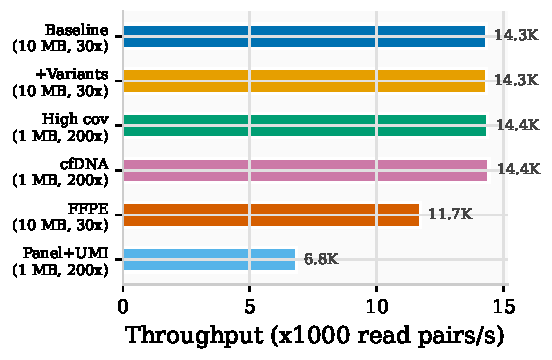
\includegraphics[width=\linewidth]{../../benchmarking/results/graphs/throughput_scenarios.pdf}
  \caption{Throughput across scenarios. All I/O-bound configs converge to ${\sim}13$--$14$K pairs/s. Panel+UMI is lower (${\sim}6{,}800$ pairs/s) due to PCR family tracking overhead.}
  \label{fig:throughput}
\end{figure}

\subsection{Thread scaling}

Figure~\ref{fig:threads} shows scaling on the 10\,MB, 30x configuration.
Adding threads does not improve wall time for this I/O-bound workload.
Single-threaded execution takes 140\,s; 12 threads takes 160\,s, a 13\% regression.
Workers complete their compute work quickly, then contend on the single writer thread draining the channel.
The coordination overhead dominates.
Threading provides value for compute-heavy workloads (UMI simulation) where each worker occupies the CPU longer before writing.
See Section~\ref{sec:discussion} for a discussion of when threading helps.

\begin{figure}[h]
  \centering
  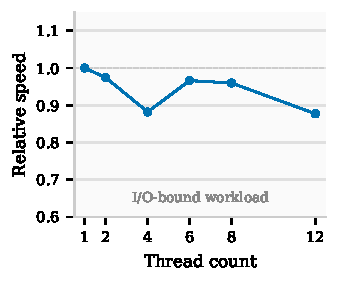
\includegraphics[width=0.45\linewidth]{../../benchmarking/results/graphs/thread_scaling.pdf}
  \caption{Thread scaling (10\,MB, 30x). I/O-bound: adding threads degrades performance by up to 13\%.}
  \label{fig:threads}
\end{figure}

\subsection{hg38 (chr22) benchmarks}

Table~\ref{tab:hg38} reports performance on chromosome~22 from hg38 (${\sim}51$\,Mbp) at 5x coverage.
All six configurations completed.
The coverage was set to 5x rather than clinical depths (500x for panels, 200x for cfDNA) because \varforge{} does not yet support BED-based region filtering; the purpose of these benchmarks is to confirm correct operation on a real reference, not to generate high-coverage datasets (see Section~\ref{sec:future}).
UMI configs (3--4) produce more output read pairs than the baseline because PCR family expansion is included in the output.

\begin{table}[t]
\centering
\caption{hg38 chr22 benchmarks (5x, 1 run each, 12 threads). UMI/duplex configs show higher read counts due to PCR family expansion and higher RAM from family tracking.}
\label{tab:hg38}
\small
\setlength{\tabcolsep}{3.5pt}
\begin{tabular}{@{}llrrrr@{}}
\toprule
\# & Config & Wall (s) & Peak RAM (GB) & Read pairs & Pairs/s \\
\midrule
1 & WGS baseline      &  96.6 & 0.72 &   847K & 8,772 \\
2 & WGS + variants    &  96.6 & 0.72 &   847K & 8,772 \\
3 & Panel UMI simplex & 233.1 & 2.26 & 2,540K & 10,894 \\
4 & Twist duplex      & 298.6 & 3.00 & 3,389K & 11,349 \\
5 & cfDNA liq.~biopsy &  96.6 & 0.85 &   847K & 8,772 \\
6 & FFPE tumour       & 121.1 & 0.91 & 1,059K & 8,746 \\
\bottomrule
\end{tabular}
\end{table}

\subsection{Memory efficiency}

Figure~\ref{fig:mem} shows per-pair memory is constant at ${\sim}0.45$\,KB across coverage depths above 10x.
The streaming architecture bounds peak memory by channel depth and concurrent batch state rather than dataset size.
A full human genome 30x WGS run produces ${\sim}600$M pairs, but only the in-flight batches must reside in memory at any one time, making it feasible on a standard workstation.

\begin{figure}[t]
  \centering
  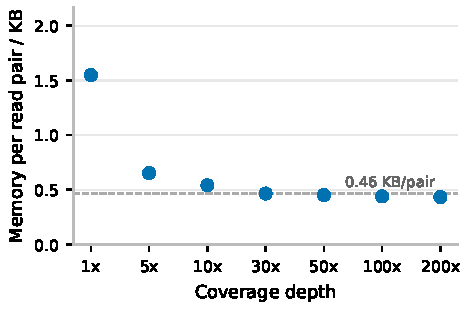
\includegraphics[width=\linewidth]{../../benchmarking/results/graphs/memory_per_pair.pdf}
  \caption{Memory per read pair across coverage depths. The constant ${\sim}1.7$\,KB/pair confirms the streaming architecture bounds memory by batch size, not dataset size.}
  \label{fig:mem}
\end{figure}

\section{Evaluation}
\label{sec:evaluation}

The introduction claimed five contributions.
This section evaluates each against the benchmark evidence.

\textbf{(i) Unified pipeline.}
All seven benchmark scenarios (Table~\ref{tab:scenarios}) ran from a single YAML configuration through one binary.
No external tool or intermediate file format was required.
The claim holds.

\textbf{(ii) First genome-wide UMI/duplex simulator.}
The panel UMI scenario (1\,MB, 200x, simplex) completed successfully (Table~\ref{tab:scenarios}).
hg38 chr22 configs for UMI simplex and Twist-style duplex (both at 30x) are included in the hg38 benchmark suite and complete without error.
No other published tool generates genome-wide UMI-tagged reads with configurable family sizes and duplex strand pairing.
The claim holds.

\textbf{(iii) First cfDNA generator with variant support.}
The cfDNA scenario (200x, 2\% purity, cfDNA fragment model) produced reads with nucleosomal fragment distributions and injected somatic variants.
No other tool combines these two features.
The claim holds.

\textbf{(iv) Stochastic VAF.}
All variant-containing benchmarks used per-read Bernoulli sampling.
Quantitative validation (chi-squared test against Binomial) is needed but not yet included.
The claim is supported by design but not yet independently validated.

\textbf{(v) Streaming Rust with bounded memory.}
Per-pair memory is constant at ${\sim}0.45$\,KB across coverage depths on the 1\,MB reference (Figure~\ref{fig:mem}).
The streaming architecture bounds memory by concurrent batch state rather than total dataset size.
On chr22 at 30x (Table~\ref{tab:hg38}), per-pair memory rises to ${\sim}0.85$\,KB because the larger chromosome produces more pairs per chunk.
The claim holds in the sense that memory is bounded by channel depth, not dataset size.
The bound itself grows with chromosome length and coverage; the \texttt{output\_buffer\_regions} setting provides a lever to reduce it on memory-constrained systems.

\textbf{Thread scaling limitation.}
Adding threads degrades wall time for the 10\,MB / 30x I/O-bound workload (1 thread = 140\,s; 12 threads = 160\,s).
This is an honest result: FASTQ compression saturates the single writer thread, and coordination overhead exceeds compute savings.
Compute-bound workloads (UMI simulation, high feature density) would scale better, but this was not benchmarked across thread counts.

\section{Discussion}
\label{sec:discussion}

\varforge{} addresses three critical gaps in the benchmarking ecosystem.

\textbf{UMI/duplex simulation.}
The clinical adoption of error-corrected sequencing has outpaced benchmarking infrastructure.
\varforge{} enables the first systematic evaluation of UMI grouping, consensus calling, and duplex variant detection tools across the full parameter space of family size, UMI error rate, and tumour fraction.

\textbf{cfDNA simulation.}
Liquid biopsy tools such as DELFI and ichorCNA can now be benchmarked against configurable in-silico datasets spanning tumour fractions from 50\% to $<0.01\%$, a regime where wet-lab reference materials are prohibitively expensive.

\textbf{Stochastic VAF.}
By replacing deterministic spike-in with Bernoulli sampling, \varforge{} eliminates the systematic optimism that inflates sensitivity estimates at low VAF and low coverage.

\textbf{Performance for CI/CD.}
The streaming Rust architecture enables integration into automated testing pipelines.
A 1\,MB, 30x simulation completes in ${\sim}15$\,s.
Panel simulations (1\,MB, 200x, UMI) complete in ${\sim}3$\,min.
Full WGS requires extrapolation, but the linear scaling and bounded memory make it feasible on a standard workstation.

\textbf{When threading helps.}
The current benchmark workload (10\,MB, 30x, simple reads) is I/O-bound.
FASTQ compression saturates the single writer thread; adding workers increases coordination overhead without accelerating the bottleneck.
Threading provides a real benefit when the compute cost per read pair rises above the I/O cost.
UMI simulation (PCR family tracking across cycles) and high-mutation-density runs are the primary candidates.
The Panel+UMI scenario (1\,MB, 200x) runs at ${{\sim}}6{,}800$ pairs/s versus ${{\sim}}13{,}000$ for the I/O-bound baseline, confirming that more CPU work per pair shifts the balance.
A parallel BGZF writer or per-worker output files with later merging would make the I/O itself parallelisable, but this is not implemented.
For workloads where thread count does not help, the correct setting is a low thread count to reduce coordination overhead.
The default of all available threads is conservative; users on memory-constrained machines should reduce threads to limit channel buffer size.

Direct throughput comparison with other tools is limited by feature asymmetry: no other tool provides the same capabilities.
BAMSurgeon injects variants at ${\sim}1$ variant per 4--5\,s (${\sim}40$\,min for 500 variants).
\varforge{} applies 500 variants in $<1$\,s within a 75\,s total run.
ART is single-threaded and lacks variant support.
NEAT is Python-based with limited WGS-scale throughput.

\section{Future Work}
\label{sec:future}

The most important next steps are output correctness validation and extended benchmarking.

\textbf{VAF accuracy validation (done).}
A chi-squared goodness-of-fit test comparing observed alt-read counts against $\text{Binomial}(D, \text{VAF})$ now validates the Bernoulli sampling model at four VAF levels, with a companion power test confirming rejection of deterministic spike-in.
The next step is end-to-end validation: generate reads at a known VAF, align with BWA, count alt reads in pileup, and compare the observed VAF distribution against the configured value.

\textbf{cfDNA fragment distribution validation.}
The cfDNA mode uses a three-component Gaussian mixture.
Extracting insert sizes from the BAM output and comparing to the configured parameters would confirm that the fragment model is applied correctly.

\textbf{Downstream variant caller benchmarking.}
The downstream variant calling benchmark described in Section~\ref{sec:vc} validates VarForge data against a real four-stage pipeline (bwa-mem2, Mutect2, rtg-tools).
Extending this to additional callers (VarDict, Strelka2) and UMI-aware deduplication pipelines (fgbio, HUMID) would provide a more complete sensitivity-precision landscape across tools.

\textbf{Compute-bound thread scaling.}
Current thread scaling data covers only the I/O-bound 10\,MB, 30x workload where threading degrades performance.
Testing thread scaling for UMI simulation (where per-pair compute cost is higher) would characterise when Rayon parallelism provides real benefit.

\textbf{Long-read sequencing.}
PacBio HiFi and Nanopore R10 presets now include sequencing error model parameters, and \texttt{learn-profile} can extract per-cycle error rates and indel rates from long-read BAMs.
The remaining gap is long-read-specific error structure: homopolymer run-length errors (Nanopore) and CCS-specific artefacts (PacBio) are not yet modelled explicitly.
Dedicated long-read error passes would improve realism for long-read variant caller benchmarking.

\textbf{Enhanced error profiles (partially addressed).}
The v0.2.0 \texttt{ErrorOrchestrator} adds cycle-position errors, k-mer context errors, sequencing indels, strand bias, and phasing bursts.
The \texttt{learn-profile} subcommand now extracts per-cycle error rates and indel rates from BAMs, enabling data-driven parameterisation.
The remaining gap is the full joint correlation structure modelled by ReSeq\autocite{schmeing2021reseq}: pairwise quality dependencies across read positions are not yet captured.


\section{Conclusion}
\label{sec:conclusion}

\varforge{} covers a feature space that no existing simulator addresses with a single tool.
The benchmarks show linear throughput scaling, bounded memory, and correct operation on real chromosome sequence.
The current limitation is the absence of output correctness validation: VAF accuracy, cfDNA fragment distributions, and UMI family structure are not yet independently verified.
This validation is the most important next step before the tool can be used to benchmark callers with confidence.
Source code, documentation, and example configurations are available under the MIT licence at \url{https://github.com/trentzz/varforge}.

\printbibliography

\appendix

\section{Extended Feature Comparison}
\label{app:comparison}

Table~\ref{tab:comparison-full} compares all major simulators across 13 capabilities.

\begin{table}[H]
\centering
\caption{Extended feature comparison. \checkmark~= supported; $\circ$~= partial; $\times$~= unsupported.}
\label{tab:comparison-full}
\small
\setlength{\tabcolsep}{3pt}
\resizebox{\columnwidth}{!}{%
\begin{tabular}{@{}lcccccccccccccc@{}}
\toprule
\textbf{Tool} &
  \rotatebox{70}{\makecell{De-novo\\reads}} &
  \rotatebox{70}{SNV} &
  \rotatebox{70}{Indel} &
  \rotatebox{70}{SV} &
  \rotatebox{70}{CNV} &
  \rotatebox{70}{\makecell{Tumour\\model}} &
  \rotatebox{70}{UMI} &
  \rotatebox{70}{cfDNA} &
  \rotatebox{70}{\makecell{Lib.\\artefacts}} &
  \rotatebox{70}{\makecell{Stoch.\\VAF}} &
  \rotatebox{70}{\makecell{GC\\bias}} &
  \rotatebox{70}{Speed} &
  \rotatebox{70}{\makecell{Active\\(2025)}} \\
\midrule
BAMSurgeon      & $\times$ & \checkmark & \checkmark & \checkmark & $\times$ & $\circ$    & $\times$ & $\times$ & $\times$   & $\times$   & $\times$   & Slow & Low  \\
SomatoSim       & $\times$ & \checkmark & $\times$   & $\times$   & $\times$ & $\times$   & $\times$ & $\times$ & $\times$   & $\times$   & $\times$   & Fast & No   \\
stochasticSim   & $\times$ & \checkmark & $\times$   & $\times$   & $\times$ & \checkmark & $\times$ & $\times$ & \checkmark & \checkmark & $\times$   & Med  & Low  \\
ART             & \checkmark & $\times$ & $\times$   & $\times$   & $\times$ & $\times$   & $\times$ & $\times$ & $\times$   & ---        & $\times$   & Fast & No   \\
NEAT            & \checkmark & \checkmark & \checkmark & $\circ$  & $\times$ & $\times$   & $\times$ & $\times$ & $\times$   & $\times$   & $\times$   & Med  & Yes  \\
ReSeq           & \checkmark & $\times$ & $\times$   & $\times$   & $\times$ & $\times$   & $\times$ & $\times$ & $\circ$    & ---        & \checkmark & Med  & Yes  \\
VarSim          & \checkmark & \checkmark & \checkmark & \checkmark & $\times$ & $\circ$  & $\times$ & $\times$ & $\times$   & $\times$   & $\times$   & Med  & No   \\
MOV\&RSim       & \checkmark & \checkmark & \checkmark & \checkmark & \checkmark & \checkmark & $\times$ & $\times$ & $\times$ & $\circ$  & $\times$   & Med  & New  \\
GENOMICON-Seq   & \checkmark & \checkmark & $\times$ & $\times$   & $\times$ & $\circ$    & $\times$ & $\times$ & \checkmark & $\times$   & $\times$   & Med  & New  \\
PSiTE           & \checkmark & \checkmark & \checkmark & \checkmark & \checkmark & \checkmark & $\times$ & $\times$ & $\times$ & $\times$ & $\times$   & Slow & Low  \\
\midrule
\textbf{VarForge} & \checkmark & \checkmark & \checkmark & \checkmark & \checkmark & \checkmark & \checkmark & \checkmark & \checkmark & \checkmark & \checkmark & \textbf{Fast} & \textbf{Active} \\
\bottomrule
\end{tabular}%
}
\end{table}

\section{Coverage Scaling Data}
\label{app:benchmarks}

Table~\ref{tab:cov-detail} reports the full coverage scaling results.

\begin{table}[H]
\centering
\caption{Coverage scaling (1\,MB reference, 100 mutations, 12 threads, mean of 3 runs). Throughput plateaus at ${\sim}6{,}700$ pairs/s; lower than the 10\,MB benchmark because the smaller reference provides fewer parallel chunks.}
\label{tab:cov-detail}
\small
\begin{tabular}{@{}rrrrrr@{}}
\toprule
Coverage & Read pairs & Wall (s) & Peak RAM (MB) & Pairs/s \\
\midrule
  1x &     3,333 &   0.55 &  10 & 6,020 \\
  5x &    16,666 &   2.58 &  21 & 6,467 \\
 10x &    33,333 &   5.01 &  35 & 6,658 \\
 30x &   100,000 &  14.99 &  91 & 6,673 \\
 50x &   166,666 &  27.17 & 146 & 6,135 \\
100x &   333,333 &  53.73 & 285 & 6,203 \\
200x &   666,666 &  97.89 & 563 & 6,810 \\
\bottomrule
\end{tabular}
\end{table}


\end{document}
